\documentclass[11pt]{article}

\usepackage{epsfig}
\usepackage{amsfonts}
\usepackage{amssymb}
\usepackage{amstext}
\usepackage{amsmath}
\usepackage{xspace}
\usepackage{theorem}
\usepackage{hyperref}
\usepackage{fullpage}
\usepackage{framed}

\usepackage{enumitem}                     
\usepackage{listings}
\usepackage{color}

\usepackage{titlesec}

\usepackage{tikz}
\usepackage{graphicx}
\usetikzlibrary{positioning}

\definecolor{dkgreen}{rgb}{0,0.6,0}
\definecolor{gray}{rgb}{0.5,0.5,0.5}
\definecolor{mauve}{rgb}{0.58,0,0.82}

\titleformat*{\section}{\bfseries}
\titleformat*{\subsection}{\bfseries}
\titleformat*{\subsubsection}{\bfseries}
\titleformat*{\paragraph}{\bfseries}
\titleformat*{\subparagraph}{\bfseries}

\newenvironment{proof}{{\bf Proof:  }}{\hfill\rule{2mm}{2mm}}
\newenvironment{proofof}[1]{{\bf Proof of #1:  }}{\hfill\rule{2mm}{2mm}}
\newenvironment{proofofnobox}[1]{{\bf#1:  }}{}
\newenvironment{example}{{\bf Example:  }}{\hfill\rule{2mm}{2mm}}

\newtheorem{fact}{Fact}
\newtheorem{lemma}[fact]{Lemma}
\newtheorem{theorem}[fact]{Theorem}
\newtheorem{definition}[fact]{Definition}
\newtheorem{corollary}[fact]{Corollary}
\newtheorem{proposition}[fact]{Proposition}
\newtheorem{claim}[fact]{Claim}
\newtheorem{exercise}[fact]{Exercise}

% math notation
\newcommand{\N}{\ensuremath{\mathbb N}}
\newcommand{\Z}{\ensuremath{\mathbb Z}}
\newcommand{\Q}{\ensuremath{\mathbb Q}}
\newcommand{\R}{\ensuremath{\mathbb R}}
\newcommand{\F}{\ensuremath{\mathcal F}}
\newcommand{\SymGrp}{\ensuremath{\mathfrak S}}

\newcommand{\size}[1]{\ensuremath{\left|#1\right|}}
\newcommand{\ceil}[1]{\ensuremath{\left\lceil#1\right\rceil}}
\newcommand{\floor}[1]{\ensuremath{\left\lfloor#1\right\rfloor}}
\newcommand{\poly}{\operatorname{poly}}
\newcommand{\polylog}{\operatorname{polylog}}

% anupam's abbreviations
\newcommand{\e}{\epsilon}
\newcommand{\half}{\ensuremath{\frac{1}{2}}}
\newcommand{\junk}[1]{}
\newcommand{\sse}{\subseteq}
\newcommand{\union}{\cup}
\newcommand{\meet}{\wedge}

\newcommand{\prob}[1]{\ensuremath{\text{{\bf Pr}$\left[#1\right]$}}}
\newcommand{\expct}[1]{\ensuremath{\text{{\bf E}$\left[#1\right]$}}}
\newcommand{\Event}{{\mathcal E}}

\newcommand{\mnote}[1]{\normalmarginpar \marginpar{\tiny #1}}


\lstset{frame=tb,
  language={},
  aboveskip=3mm,
  belowskip=3mm,
  showstringspaces=false,
  columns=flexible,
  basicstyle={\small\ttfamily},
  numbers=none,
  numberstyle=\tiny\color{gray},
  keywordstyle=\color{blue},
  commentstyle=\color{dkgreen},
  stringstyle=\color{mauve},
  breaklines=true,
  breakatwhitespace=true,
  tabsize=3
}

\definecolor{codegray}{gray}{0.9}
\newcommand{\code}[1]{\texttt{#1}}
\newcommand{\codebox}[1]{\colorbox{codegray}{\texttt{#1}}}

\setenumerate[0]{label=\arabic*.}

\newlength\tindent
\setlength{\tindent}{\parindent}
\setlength{\parindent}{0pt}
\renewcommand{\indent}{\hspace*{\tindent}}

\graphicspath{{./}}

%%%%%%%%%%%%%%%%%%%%%%%%%%%%%%%%%%%%%%%%%%%%%%%%%%%%%%%%
% Document begins here %%%%%%%%%%%%%%%%%%%%%%%%%%%%%%%%%%%%%%%%%%%
%%%%%%%%%%%%%%%%%%%%%%%%%%%%%%%%%%%%%%%%%%%%%%%%%%%%%%%%

\begin{document}

\noindent {\bf{HUGH HAN, ANISH DALAL} \vspace{4pt} \\ \large {\bf 600.465 Natural Language Processing} \hfill {{\bf Fall 2016}}}\\
{{\bf Homework \#4}} \hfill {{\bf Due:} 26 October 2016, 2:00pm} \vspace{6pt} \\
\rule[0.1in]{\textwidth}{0.4pt}

\begin{enumerate}
\item % PROBLEM 1
	For this problem, we decided to use the Berkeley parser.
	\begin{enumerate}[label=(\alph*)]
	\item
		One interesting thing about the style of the trees the vast number of symbol types that it has. It represents the different types of words in the English language very well.

		What we thought was particularly cool was that if you gave the parser some gibberish words, it would either
		\begin{enumerate}[label=(\roman*)]
			\item
				Classify those gibberish rules as plain ``symbols'' if it didn't have enough contextual information to make a guess (for example when there is only one word),
			\item
				Make an educated guess on what types of words the gibberish actually is.  That is, it guesses the most probable parse rules that could lead to this type of sentence, based contextual information.

				We think that the contextual information could be things such as the number of words or the words surrounding unrecognized words.
		\end{enumerate}
		Consider the following nonsensical sentence.
		\begin{eqnarray*}
			\codebox{My asdfjkasdjl went alksdf the store}
		\end{eqnarray*}
		After reading that sentence, the parser deduced that the structure would look something like the following.

		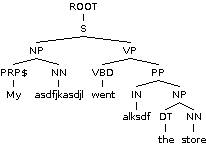
\includegraphics[scale=0.7]{gibparsetree.png}
		
	\item

		From our examples, it would seem that any sentence that contained syntactic or lexical ambiguity statements caused the parser to produce an incorrect parse.

		We tried feeding the following sentence into the parser:
		\begin{eqnarray*}
		\codebox{Buffalo buffalo Buffalo buffalo buffalo buffalo Buffalo buffalo}
		\end{eqnarray*}
		The output produced was the following.
		\begin{lstlisting}
		(ROOT
		  (NP
		    (NP (NNP Buffalo) (NNP buffalo) (NNP Buffalo))
		    (NP (JJ buffalo) (NN buffalo) (NN buffalo) (NNP Buffalo) (NNP buffalo))))
    	\end{lstlisting}
    	Note that there is no NP VP clause, when there really should be. That is, the word buffalo can behave as a verb, and the parser fails to recognize this.

\newpage

    	We can also think of the following sentence:
    	\begin{eqnarray*}
    	\codebox{James while John had had had had had had had \ } \\
    	\codebox{had had had had a better effect on the teacher}
    	\end{eqnarray*}
    	When fed into the parser, the following parse is generated.
    	\begin{lstlisting}
		(ROOT
		  (S
		    (NP (NNP James) (IN while) (NNP John))
		    (VP (VBD had)
		      (VP (VBN had)
		        (S
		          (VP (VBD had)
		            (VP (VBD had)
		              (VP (VBD had)
		                (VP (VBD had)
		                  (VP (VBD had)
		                    (VP (VBD had)
		                      (VP (VBD had)
		                        (S
		                          (VP (VBD had)
		                            (VP (VBN had)
		                              (NP
		                                (NP (DT a) (JJR better) (NN effect))
		                                (PP (IN on)
		                                  (NP (DT the) (NN teacher)))))))))))))))))))
    	\end{lstlisting}

		Next, we thought of the following sentence.
    	\begin{eqnarray*}
    		\codebox{If police police police police, who police police police?}
    	\end{eqnarray*}

    	Below is its parse tree.

    	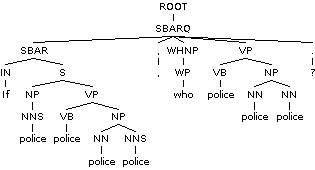
\includegraphics[scale=0.7]{policepoliceparsetree.png}

		The way the sentence is structured, it is referring to a noun phrase ``police police" who are in charge of ``police". The sentence is saying ``If there are police officers who monitor other police officers who monitors those police officers?". The parser got the ``police police" noun phrase correct in the second half of the sentence but failed to recognize ``police police" as a noun phrase in the first half (it believes ``police" police ``police police", rather than ``police police" police ``police").  

		The parser does not handle garden path sentences very well either. However, it managed to produce the correct parse for ``The complex houses married and single soldiers and their families"

		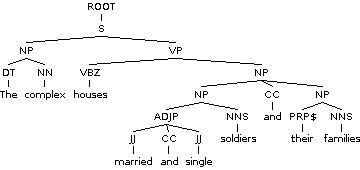
\includegraphics[scale=0.7]{gardenpath.png}

	\item

		We created the following grammatical sentence.
		\begin{eqnarray*}
			\codebox{Buffalo run runs running runs} 
		\end{eqnarray*}

		The sentence contains lexical ambiguity. It means ``Buffalo run their runs while running their runs". The phrase ``running runs" is a VP and an NP, so it should be created from the following rule.
		\begin{eqnarray*}
			\texttt{VP} \rightarrow \texttt{VP NP}
		\end{eqnarray*}rule. 
		The parser incorrectly parses this since it makes the phrase ``running runs" an \texttt{NP}.

		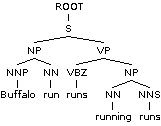
\includegraphics[scale=0.7]{buffalorun.png}

		Finally we searched for a sentence online. We found the following sentence.

		\begin{eqnarray*}
			\codebox{The word of the Lord came to Zechariah, son of Berekiah, son of Iddo, the prophet}
		\end{eqnarray*} 
		The ambiguity is that ``the prophet" can refer to either ``Iddo" or ``Zechariah" when in reality it refers to ``Zechariah" (this sentence is from the hebrew Bible). The parser believes the Iddo is the prophet rather than Zechariah. In the parse below, it creates a noun phrase for ``Iddo the prophet".

		Below is the parse tree from Berkeley.

		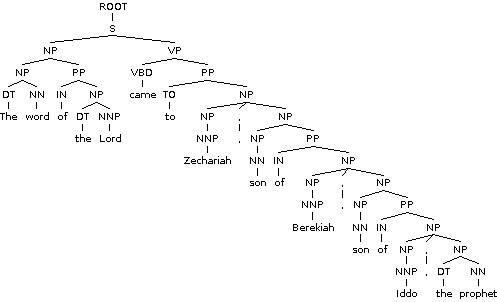
\includegraphics[scale=0.7]{zechariah.png}

	\end{enumerate}

\item
	\begin{enumerate}[label=(\alph*)]
	\item
		Our algorithm does not take more than $O(n^2)$ space. We maintain a chart of length $n+1$ where $n$ is the length of the sentence. At most, a column $j$ will have O($j$) entries, so in the worst case you have O($n+1$) entries in the last column. Now note that the following statement is true.
		\begin{eqnarray*}
			O(n+1) + O(n) + O(n-1) + O(n-2) \dots &=& O(n^2)
		\end{eqnarray*} 
		The extra space used for each column is a set (implemented by a dict) of the same size as the column. We maintain a "table entry" object which maintains the same information as a dotted rule but in a more efficient structure. 

		Our algorithm does not take more then $O(n^3)$ time. For any given rule in the chart, We either scan, predict, or complete. Scan is a $O(1)$ check against the input sentence. Predict adds all associated rules to the chart which is $O($number of rules for a non terminal$)$, and we maintain a hash map of rules in the current column to do $O(1)$ checking of duplicate rules before adding. Thus the runtime is bounded by the runtime of predict and complete. Complete similarly attaches constituents to customers. Due to the $O(1)$ check for duplicates (as well as $O(1)$ attachment as will be discussed in the next section), the runtime does not exceed $O(n^3)$.
	\item 
		We do not exceed $O(1)$ runtime for attaching to a column. We use primitive python's list object which is essentially a vector that allows $O(1)$ append to the end of the list. The list represents a column and the chart is a list of lists. There is not a time where we add to the middle of the list, so elements will not need to be shifted.
	\item 
		In the ``attach" portion of our parse method, we update weights accurately by having a table entry maintain the current weight of its own parse tree. If a rule is added by prediction, the weight assigned to it is the $\log_2 {p(}$probability of rule given by the grammar $)$. When we attach a constituent to its customer, we update weights by first adding the weight of the constituent to the weight of the customer (all weights are ``current weights" since they represent the weight of that parse) and checking if the parse tree formed is unique. If it is unique, it is added to the current column, else it is checked against the table entry for which it is the same. If the ``new" weight is less than the weight of the table entry already in the table, the old entry is removed (nullified rather than removing so that no elements need to be shifted). Thus, weights are maintained properly because they are updated when constituents are attached to customers (weight of a tree is the sum of weight of its branches) and compared against existing entries to find the optimal parse (a dynamic programming paradigm where you choose the optimal solution between two previous solutions). \\
	\end{enumerate}

\item 

	Our output from \texttt{parse2.py} is pasted below.

	\begin{lstlisting}
(ROOT (S (NP (NPR (NNP John)))
         (VP (VBZ is)
             (ADJP-PRD (JJ happy)))
         (PUNC. .)))
34.224010618
(ROOT (S (NP (DT The)
             (ADJP (RB very)
                   (JJS biggest))
             (NNS companies))
         (VP (VBP are)
             (RB not)
             (ADVP (RB likely))
             (VP (TO to)
                 (VP (VB go)
                     (PP (IN under)))))
         (PUNC. .)))
104.909225647
(ROOT (S (NP (DT The)
             (NN market))
         (VP (VBZ is)
             (VP (VBG wondering)
                 (SBAR (WHNP (WP what))
                       (S (NP (NPRS (NNP General)
                                    (NNPS Motors)))
                          (VP (VBZ has)
                              (VP (VBN done)))
                          (PUNC. .)))))))
94.5811848825
(ROOT (S (PP (IN In)
             (NP (JJ recent)
                 (NNS years)))
         ,
         (NP (NN pay))
         (VP (VBD surged)
             (SBAR (IN as)
                   (S (NP (NN demand))
                      (VP (VBD rose)
                          (SBAR (IN while)
                                (S (NP (NNS workers))
                                   (VP (VBN left)
                                       (PP (IN for)
                                           (NP (JJR easier)
                                               (NNS jobs))))))))))
         (PUNC. .)))
161.818960465
(ROOT (S (S-ADV (VP (VBN caught)
                    (PRT (RP off))
                    (NP (NN guard))))
         ,
         (NP (NPR (NNP Ford)
                  (NNP Motor)
                  (NNP Co.)))
         (VP (VBD had)
             (NP (DT no)
                 (NN choice))
             (PP (IN except)
                 (S-NOM (VP (TO to)
                            (VP (VB follow)
                                (NP (NN suit))))))
             (PP (IN with)
                 (NP (NN financing)
                     (NNS deals))))
         (PUNC. .)))
191.390539461
(ROOT (S (NP (NNS data))
         (VP (VBP show)
             (SBAR (WHNP (WDT that))
                   (S (VP (VB pay)
                          (VP (VBD was)
                              (ADJP-PRD (JJ flat)
                                        (PP (IN for)
                                            (NP (NP (DT the)
                                                    (JJ third)
                                                    (JJ consecutive)
                                                    (NN quarter))
                                                (PP (IN after)
                                                    (NP (DT a)
                                                        (NN rash))))))
                              (PP (IN of)
                                  (NP (QP (QP (CD 4))
                                          (NN %)
                                          (PP (TO to)
                                              (NP (QP (CD 5))
                                                  (NN %))))
                                      (JJ annualized)
                                      (NNS increases))))))))
         (PUNC. .)))
212.54526591
	\end{lstlisting}
	Unfortunately, we couldn't finish letting it run in time, so did not submit outputs for sentences 7, 8, or 9. However, our first 6 sentences are correct, and we are somewhat confident that 7, 8, 9 will also be correct if given enough time to run.

	To measure speedup, we ran our parser on 3 different grammars: \texttt{wallstreet.gr}, \texttt{papa.gr}, and \texttt{arith.gr}. For \texttt{wallstreet.gr}, due to how large it is, we a) ran it using pypy and b) measured speedup only on the first 3 sentences.

	\begin{center}
	\begin{tabular}{|c|c|c|}
	\hline 
	Grammar & Runtime parse.py (s) & Runtime parse2.py (s) \\ 
	\hline 
	\texttt{papa.gr} & 0.07 & 0.04 \\ 
	\hline 
	\texttt{arith.gr} & 0.05 & 0.04 \\ 
	\hline 
	\texttt{wallstreet.gr} & 98.36 & 45.28 \\ 
	\hline
	\end{tabular} 
	\end{center}

	Clearly \texttt{parse2.py}---our optimized version---runs much faster than parse.py (more than twice as fast on \texttt{wallstreet.gr}). 

	For this part, we just implemented some easy speedup tricks.

	Two speedup methods were used.
	\begin{enumerate}
		\item
			When the predict method is called, we check in constant time whether the rules for a given non-terminal have already been predicted. That is, we keep track of them. 

			If we're about to predict a batch of several hundred \texttt{NP} rules (all rules of the form \texttt{NP} $\to$ \texttt{. BLAH BLAH}), then our program first does a quick check to discover whether we've already added that batch to the current column.

			To do this, we can simply check the left-hand-side of whatever rule we're adding, and that will correspond to the same batch of rules during prediction.
		\item
			We implement rudimentary one word lookahead. When predicting, we want to avoid adding preterminals or rules whose right hand sides begin with a terminal whose terminals do not match the current word in the sentence we wish to parse. If we are trying to parse "ate", we want to avoid rules like V $\rightarrow$ observed or X $\rightarrow$ observed Y. Additionally, we want to avoid rules that will not lead to the preterminals we would like to include. For example, since we are looking for V $\rightarrow$ ate, we want rules whose right hand sides are immediately trying to parse V. Thus, we can exclude NP $\rightarrow$ NP VP. We don't see incorrect parses for \texttt{wallstreet.gr} because we don't implement pruning methods. Thus, we don't exclude low probability rules without testing them against duplicate constituents. 
	\end{enumerate}

\end{enumerate}

\end{document}
